% \graphicspath{{../figures/}{./gfx/}{/media/data/Work/cnstellate/}{/media/data/Work/cnstellate/Responses/}}

% \renewcommand{\setthesubsection}{\Alph{subsection}}
\section{Appendix    \label{sec:ch3:appendix}}

\subsection{General neural modeling tools}

This section provides an overview of the pragmatic details of the \textsf{cnstellate} NEURON model used in this chapter.

\subsubsection{Optimisation}

The optimisation routine used in this chapter was NEURON's \textsf{fit\_praxis},
which uses the algorithm PRAXIS~\citep{Brent:1976}.

\begin{lstlisting}[label=lbl:runprax,caption=Set optimisation attributes and run fitting procedure.]
-----parameters_****.hoc--------------
  NPARAMS=3
  objref pvec,fvec,pvec_ranges,pvec_name,pvec_factor
  pvec = new Vector()                // contains the parameters to be fitted
  pvec_ranges= new Matrix(NPARAMS,2) // (min,max) pairs for each param
  pvec_name = new List()             // names of parameters in String list
  pvec_factor = new Vector(NPARAMS,1)// regulates variables so pvec is in same range to aid fit_praxis
  //min
  for i=0,NPARAMS-1 pvec_ranges.x[i][0]= 0.000001
  //max
  for i=0,NPARAMS-1 pvec_ranges.x[i][1]= 0.03
  //Names                                               //Initial values	//Param Factor
  pvec_name.append(new String("param.w.x[lsr][tv]"))	pvec.append(0.00190)	pvec_factor.append(1)
  pvec_name.append(new String("param.w.x[hsr][tv]"))	pvec.append(0.00130)	pvec_factor.append(1)
  pvec_name.append(new String("param.w.x[hsr][ds]"))	pvec.append(0.00170)	pvec_factor.append(1)
---------------------
  proc runprax(){
    attr_praxis(0.0001, 0.01, 3)
    fit_praxis(NPARAMS,"error_fcn",&pvec.x[0])
  }
\end{lstlisting}


\subsubsection{Data extraction    \label{sec:data-extraction}}

\todo[inline]{Special comments on the use of g3data to extract data points from  PDF literature documents }



\begin{figure}[htb]
  \begin{center}
    \resizebox{5in}{!}{\includegraphics{NoFigure}}
    \caption{Extracting experimental data in references using g3data.}
    \label{fig:Extractdata}
  \end{center}
\end{figure}


\subsection{\textsf{cnstellate} NEURON model    \label{sec:cnstellate-neur-model}}

The cochlear nucleus stellate microcircuit software code used in this chapter is
called \textsf{cnstellate} and is implemented in NEURON, NMODL and C source
code.  Acknowledgments should be made to M.S.A. Zilany and colleagues for their
work on the AN model, Dominic Mazzoni for the real-time resample library
interface, and \citet{MiglioreCanniaEtAl:2006} for the parallel NEURON network
model \textsf{netmod} (see SenseLab models


\href{http://senselab.med.yale.edu/senselab/modeldb/ShowModel.asp?model=52034}{52034},
\href{http://senselab.med.yale.edu/senselab/modeldb/ShowModel.asp?model=2730}{2730},
\href{http://senselab.med.yale.edu/senselab/modeldb/ShowModel.asp?model=51781}{51781}).



From the command line type:
\begin{verbatim}
    $ make gui
    $ ./gui/special TStellate.hoc -
\end{verbatim}
\noindent in the \textsf{cnstellate} directory to simulate the optimisation for the T~stellate model simulation and optimisation.
The \textsf{make gui} command calls the standard \textsf{nrnivmodl} to convert all *.mod files in the directory to a compiled library, that can be imported into NEURON; then appends the \textit{libresample} interface to the locally compiled NEURON executable \textit{special}.

The first run of a stimulus may take some time if the AN responses have not been previously saved, since the Zilany \& Bruce version 3 model requires 500~kHz resolution in the stimulus, this is then downsampled to a lesser resolution for the spike generator and saved for further use.
The resolution spike generator is generally at or above 10~kHz to match the simulations' time step of 0.1 ms.  Version 4 of the AN model \citep{ZilanyBruceEtAl:2009} only needs 200~kHz sampling rate for stimulus above 20~kHz, otherwise use 100~kHz.
%The directory for the saved AN responses is determined by the variable \textsf{ANsoundspath}.



List~\ref{lst:headerlines}
\begin{lstlisting}[label=lst:headerlines,caption={Headerlines in \mbox{\textsf{TStellate\.hoc}} show a typical setup in a \textsf{cnstellate} simulation or optimisation file.}]
load_file("nrngui.hoc")
//load_file("par_netpar.hoc")     //uncomment for parallel mode
//load_file("par_init.hoc")       //uncomment for parallel mode
load_file("mathslib.hoc")       //mathematical procedures from netmod
load_file("Params.hoc")         //default parameters for cnstellate
load_file("Utilities.hoc")      //My utility functions
load_file("NetworkParameters.hoc") //NetworkParameter class
load_file("AuditoryNerve.hoc")  //ANChannel and AuditoryNerve classes
load_file("par_CNcell.tem")     //CNCell and Golgicell class

//Previous optimisation parameters
xopen("pvec_Golgi_RateLevel.hoc")
xopen("pvec_DS_ClickRecovery.hoc")
xopen("pvec_TV_Notch.hoc")

//Model parameters unique to current simulation
xopen("parameters_TStellate.hoc")

//Setup CN Stellate Network model
load_file("CochlearNucleus.hoc")    //Cells and network defined
// xopen("par_CochlearNucleus.hoc") // Model setup for parallel mode

//Create CN model
create_cells()
connect_cells()
connect_CNcells()

//Experiment routines
load_file("par_experiment_TStellate.hoc")
...
\end{lstlisting}




\subsubsection{Auditory nerve and input utilities} \label{sec:APDX:auditory-nerve-input}

The auditory model implementation in NEURON is a conversion from the MATLAB mex
interface to NEURON's NMODL interface. Version 3 of the AN model
\mbox{\textsf{an\_bruce.mod}}

Support for simulating the rat and human species, as well as the default cat
species, are included in the NMODL files \mbox{\textsf{an\_bruce.mod}} and
\mbox{\textsf{an\_zilany\_v4.mod}}.  Accommodation of different species is
implemented within the procedures \mbox{\textsf{cochlea\_x2f()}},
\mbox{\textsf{cochlea\_f2x()}}, \mbox{\textsf{delay\_species()}} occurs at the
position on the basilar membrane to characteristic frequency mapping function
(\mbox{\textsf{cochlea\_x2f()}}), the reciprocal frequency to position function
(\mbox{\textsf{cochlea\_f2x()}}), and the delay function
(\mbox{\textsf{delay\_species()}}).  Figure~\ref{fig:GetAudiogram} shows how
audiograms from the appropriate species are mapped using a MATLAB routine
\mbox{\textsf{fitaudiogram.m}} so that specific parameters can be passed from
NEURON to the auditory model.  Rat basilar membrane frequency mapping in
\mbox{\textsf{cochlea\_f2x()}} and \mbox{\textsf{cochlea\_x2f()}} included using
data obtained from the Boston University Earlab website,
\url{http://earlab.bu.edu}.  Compression variables for the IHC and OHC
components of the Zilany model are fit using audiogram data of a rat.  The
audiogram in Fig.~\ref{fig:AudThresholdCatRat} was used to generate the
compression data for the rat model.

%\smallskip{}

Listing~\ref{lst:makeaudiogram} shows the MATLAB/GNU Octave commands to get the correct Zilany model compression values, given the acoustic thresholds of an animal.
\begin{lstlisting}[label=lst:makeaudiogram,caption=Using \mbox{\textsf{fitaudiogram.m}} to create COHC and CIHC vectors for the cat.]
  x=dlmread("heffner_1985a_felis_p347_3.txt",'\t',2,0);
  [Cohc,Cihc,OHC_Loss]=fitaudiogram(x(:,1),x(,2));
  dlmwrite("cat_audiogram.txt",[x co' ci'],'\t',0,0,"precision","%g");
\end{lstlisting}



% \begin{lstlisting}[label=lst:cataudiogram,caption=Portion of  \mbox{\textsf{cat\_audiogram\.txt}}]
%   ...  125 37 0 0.025 250 22 0 0.3 500 8 0.65 0.7 1000 3 0.9 0.9 2000 1 0.95 1
%   4000 1 0.95 1 ...
% \end{lstlisting}
\begin{lstlisting}[label=lst:getaudiogramdata,caption= Procedure to get audiogram data and interpolate to frequencies in \textsf{cf} vector (\mbox{\textsf{Utilities.hoc}})]
objref audiogram,cohc,cihc
proc GetAudiogramData(){
...
  file.ropen(audiogram_file)
  audiogram.scanf(file,nrows,4)
...
  // Interpolate audiogram to frequencies in cf vector
  cohc.interpolate(cf, audiogram.getcol(0).c, audiogram.getcol(2).c)
  cihc.interpolate(cf, audiogram.getcol(0).c, audiogram.getcol(3).c)
}
\end{lstlisting}

A procedure in \mbox{\textsf{cochlea\_x2f()}} included using data obtained from
the Boston University Earlab website, \url{http://earlab.bu.edu}.
Compression variables for the IHC and OHC components of the Zilany
model are fit using audiogram data of a rat.  The audiogram in
Fig.~\ref{fig:AudThresholdCatRat} was used to generate the compression
data for the rat model.

%\smallskip{}

Listing~\ref{lst:makeaudiogram} shows the MATLAB/GNU Octave commands in
\begin{lstlisting}[label=lst:makeaudiogram,caption=Using \mbox{\textsf{fitaudiogram.m}} to create COHC and CIHC vectors for the cat.]
  x=dlmread("heffner_1985a_felis_p347_3.txt",'\t',2,0);
  [Cohc,Cihc,OHC_Loss]=fitaudiogram(x(:,1),x(,2));
  dlmwrite("cat_audiogram.txt",[x co' ci'],'\t',0,0,"precision","%g");
\end{lstlisting}



% \begin{lstlisting}[label=lst:cataudiogram,caption=Portion of  \mbox{\textsf{cat\_audiogram\.txt}}]
%   ...  125 37 0 0.025 250 22 0 0.3 500 8 0.65 0.7 1000 3 0.9 0.9 2000 1 0.95 1
%   4000 1 0.95 1 ...
% \end{lstlisting}
\begin{lstlisting}[label=lst:getaudiogramdata,caption= Procedure to get audiogram data and interpolate to frequencies in \textsf{cf} vector (\mbox{\textsf{Utilities.hoc}})]
objref audiogram,cohc,cihc
proc GetAudiogramData(){
...
  file.ropen(audiogram_file)
  audiogram.scanf(file,nrows,4)
...
  // Interpolate audiogram to frequencies in cf vector
  cohc.interpolate(cf, audiogram.getcol(0).c, audiogram.getcol(2).c)
  cihc.interpolate(cf, audiogram.getcol(0).c, audiogram.getcol(3).c)
}
\end{lstlisting}

A procedure in \mbox{\textsf{Utilities.hoc}} called  \mbox{\textsf{GetAudiogram()}} is used
to get the MATLAB/Octave audiogram data and then interpolate the data
to centre frequencies in network's frequency channels.

\begin{figure}[th]
  \begin{center}
    \resizebox{0.8\textwidth}{!}{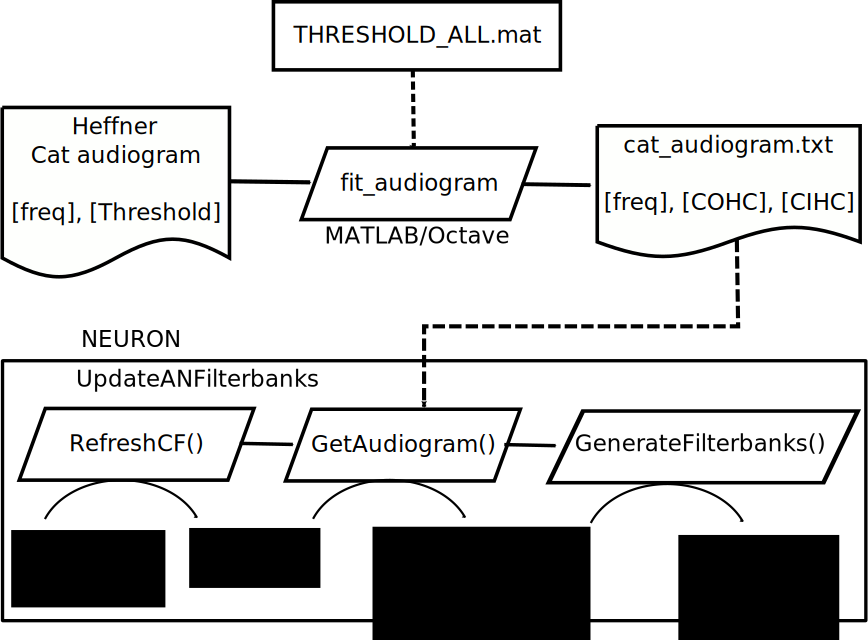
\includegraphics[keepaspectratio=true]{getaudiogram}}
    \caption[Zilany auditory model conversion in NEURON]%
    {Getting audiogram compression values for Zilany model in
      NEURON\@.  Data file
      \mbox{\textsf{``heffner\_1985a\_felis\_p347\_3.txt''}} (obtained
      from [earlab.bu.edu]) is used in \textsf{fitaudiogram.m} to
      generate outer and inner hair cell compression values.  When
      used in the \textsf{cnstellate} model in NEURON, the compression
      values are interpolated to frequency positions in the
      \textsf{cf} vector.
\label{fig:GetAudiogram}}
  \end{center}
\end{figure}

\begin{figure}[htb]
  \begin{center}
\resizebox{0.9\textwidth}{!}{\includegraphics{gfx/Audiogram_COHC_CIHC_cat}%
\includegraphics{gfx/Audiogram_COHC_CIHC_rat}}
%    \resizebox{0.5\textwidth}{!}{\includegraphics[keepaspectratio=true]{NoFigure}}
%\resizebox{0.6\textwidth}{!}{\includegraphics[keepaspectratio=true]{audiograms}}
\caption[Audiogram and compression in rats and cats]%
{Hearing threshold audiogram of the domestic cat by
  \citet{HeffnerHeffner:1985} (A) and the Norwegian rat by
  \citet{HeffnerHeffner:1985} (B).  (Data obtained from
  \href{earlab.bu.edu}).  Compression values for the Zilany AN model
  for cat (C) and rat (D).}
\label{fig:AudThresholdCatRat}
  \end{center}
\end{figure}


%\smallskip{}

The formula for the latency of acoustic stimulation to reach a
particular point on the basilar membrane comprises a fixed conduction
delay plus an additional delay that is an exponential function of the
distance from the stapes.  The frequency mapping function is defined
as:
\begin{equation}
  \label{eq:BM}
  f(x) = A\times10^{\left(a * x / L\right)} - K
\end{equation}
\noindent where \emph{x} is distance along the basilar membrane from
the stapes.

%\smallskip{}

This equation is suitable since it uses the mapping function
\mbox{\textsf{cochlea\_x2f()}} and its inverse,
\mbox{\textsf{cochlea\_f2x()}}, which is different for cat, rat and
humans.  The data listed in Table~\ref{tab:f2x} shows the currently
accepted parameters for each species.


\begin{table}[ht]
  \centering
  \begin{tabular}{lccccc}
  \hline
% after \\: \hline or \cline{col1-col2} \cline{col3-col4} ...
      &   A  &  a   &     k     & L \\
Human & 165.4 & 2.1  & 1.0(0.88) & 35\\
 Cat  &  456  & 2.1  &    0.8    & 25 \\
 Rat  & 7613.3& 0928 &    1.0    & 8.03 \\
  \hline
  \end{tabular}
  \caption[Basilar membrane frequency-distance function parameters]%
  {Frequency to basilar membrane distance function parameters \citep{FitzGeraldBurkittEtAl:2001}. Data obtained from \url{http://earlab.bu.edu} \label{tab:f2x}}
\end{table}


In the cat, \citet{CarneyYin:1988} fitted the latency vs \CF~curve
from click responses in the cat to obtain the equation:
\begin{equation}
  \label{eq:delay}
   delay (x) = A_0 * {\rm exp}(-x / A_1 ) * 1e-3 - 1.0/CF
\end{equation}
\noindent where $x = \mathsf{cochlea\_f2x(species, CF)}$ is the
distance along the basilar membrane, $A_0 = 8.13$ ms, $A_1 = 6.49$ nm.
\citet{HeinzZhangEtAl:2001} then corrected the peak click to match the
onset delay of ANFs and this has been retained in the model used here
\citep{ZilanyBruceEtAl:2009}: \(delay = A_0 * {\rm exp}(-x / A_1) *
1e-3 \) where $A_0 = 3.0$, $A_1 = 12.5$. In humans, the delay function
is: \( delay = 4.915 + 0.3631 * {\rm exp}(0.11324*x),\quad 5<x<35 (mm)
\).

%\smallskip{}

Steps for converting any Carney Auditory Model written in C~for MATLAB~to a NEURON~NMODL~compatible C~file.
\begin{enumerate}
\item Remove mex headers
\item remove \textsf{mexfunction}, this is replaced with equivalent NMODL function that retrieves variables and returns the equivalent vectors
\item Find and replace all vector or memory allocation routines with functions in scopmath.h
  \begin{itemize}
  \item \textsf{mxCalloc}$\Rightarrow$\textsf{makevector}
  \item \textsf{mxFree} $\Rightarrow$ \textsf{freevector}
  \end{itemize}
\item Replace random generator functions \textsf{drand48()} to \mbox{\textsf{scop\_random()}} and let random seed be set in NEURON or replace \textsf{srand(seed)} with \mbox{\textsf{set\_seed(seed)}}.
\item Calls to MATLAB functions within a mex file The most recent model within the mex file.  This was converted to a simple double array of random values with the \protect{\mbox{\textsf{normrand(0,1)}}} function in \mbox{\textsf{scoplib.h}}.
  \begin{itemize}
  \item builtin \textsf{randn} $\Rightarrow$ generate an array gaussian random numbers with scoplib's \mbox{\textsf{normrand(0,1)}} function
  \item builtin \textsf{resample} $\Rightarrow$ implementation of a reliable resampling function in C, using a real-time resample library (libresample [reference needed]).
  \item M-file \textsf{ffGn} $\Rightarrow$ generate a C function that implements a the fast fractional Gaussian noise generator
  \end{itemize}
\end{enumerate}


\subsection[Spiking model]{ANF spiking model}

The spike generator used in the CN stellate model was created by
B. Scott Jackson (bsj22@cornell.edu).  The code is available from the
Carney Lab web site
\href{http://www.urmc.rochester.edu/smd/Nanat/faculty-research/lab-pages/LaurelCarney/auditory-models.cfm}.

The double exponentials for the refractory recovery, specific to ANFs,
were:
\begin{eqnarray}
y_0(t) = c_0*exp(-t/s_0) \\
y_1(t) = c_1*exp(-t/s_1) \\
\end{eqnarray}
where $t$ is the time relative to the last spike, $c_0 = 0.5$, $c_1 =
0.5$, $s_0 = 0.001$ ms, and $s_1 = 0.0125$ ms.  The absolute dead time
was 0.00075 seconds.





\subsection[CN cells]{Cochlear Nucleus Cell Templates }

%\yellownote{RM NMODL files}
%\citep{RothmanManis:2003b}

The cochlear nucleus cell models were introduced by \citet{RothmanManis:2003b}, after exploratory studies on the potassium currents of murine cochlear nucleus neurons \citep{RothmanManis:2003,RothmanManis:2003a}.
Listing~\ref{lst:CellTemplate} shows the basic cell template for the single compartment neural models in the CN stellate microcircuit.
Each neuron contains a NEURON segment called soma that contains the active currents, synapses receptors and a spike detector. The model can be adjusted to include dendrite and axon segments if required.
Internal variables and objects can be made publicly accessible using

The \sf{rm} module loaded for each \textsf{CNcell} soma section is the condensed current modules of sodium (\sf{Na}), high-threshold potassium (\sf{KHT}), leak, and the hyperpolarising mixed-cation (\sf{Ih}).
The low-threshold potassium current module (KLT), is only used by the \DS~cell and inserted seperately.

\begin{lstlisting}[label=lst:CellTemplate,caption=Rothman and Manis cochlear nucleus cell template (in CNcell.tem)]
  begintemplate CNcell
  public soma, dend        //NEURON sections
  public AMPA, GlyR, GABAA //synapse objects
  public spikes,spiketimes //storage vectors
  public connect2target, synlist //synapse connection function and list
  public cf,model,channel //identifying parameters
...
  proc init(){local model
    create soma //primary section
    synlist = new List()
    spiketimes = new Vector()
    spikes = new Vector()
    //Cell type mode
    if($1 == 0) set_tstellate() //T~stellate cell
    if($1 == 1) set_tuberc()    //Tubervuloventral cell
    if($1 == 2) set_dstellate() //D~stellate cell
    if($1 == 3) set_golgi() //Golgi cell
    cf = $2
    channel=$3

    soma {
//insert Rothman and Manis default currents (Na, KHT, Ih, and leak)
      insert rm
//insert AMPA Excitatory synapse
      AMPA = new ExpSyn(0.5)
      AMPA.tau = ampa_decay
      AMPA.e = ampa_erev
//insert Glycinergic inhibitory synapse
      GlyR = new Exp2Syn(0.5)
      GlyR.tau2 = gly_decay
      GlyR.tau1 = gly_rise
      GlyR.e = gly_erev
//insert GABA-A inhibitory synapse
      GABAA = new Exp2Syn(0.5)
      GABAA.tau2 = gaba_decay
      GABAA.tau1 = gaba_rise
      GABAA.e = gaba_erev
    }
    // Set reversal potentials
    soma.eleak_rm = Erest          //mV, Leak reversal potential mV
    soma.eh_rm = -43         //mV, reversal potential for Ih
    ena = 50 // mV
    ek = -70 // mV
 }//init
...

proc set_tstellate() {
   model = 0
   soma {
     insert ka
     Ra   = 150            //axial resistance per cm
     cm   = 0.9            //micro farad per cm^2, membrance capacitance
     L    = 19.5           //length of cell body
     diam = L              //diameter of cell body
     somaarea = PI*(L/1E4)^2   //um to cm2

//Set maximum conductance for each current
	gnabar_rm = nstomho(1000)*qt()
	gkhtbar_rm = nstomho(80)*qt()
	gkabar_ka =  nstomho(65)*qt()
	ghbar_rm = nstomho(0.5)*qt(1)
	gleak_rm = nstomho(2)*qt()
   }
}
endtemplate CNcell

\end{lstlisting}



\subsubsection[Golgi model]{Golgi cell model
  optimisation    \label{sec:APDX:golgi-cell-model}}

Each golgi cell template consists of a spike generator, \emph{sg}, a
vector object representing the instantaneous rate, and a vector object
of the current spike times and a list of accumulated spike times in
previous repetitions.  The spike generator is the same inhomogeneous
Poisson point process as used in the ANF spiking models.  Parameters
identifying each cell include the \emph{channel} number, CF and
bandwidth of ANF input (actually the variance of the weight each
auditory filter channel contributes to the firing of the cell).

The rate-based golgi cell model at CF channel \emph{i} is created by:
\begin{itemize}
\item a selection of ANF input channels centred at \emph{i} with
  variance $\sLSRGLG/2$;
\item the instantaneous rate vectors of the LSR ANF's in each channel
  are weighted (with a gaussian function (mean=\emph{i}, standard
  deviation = $\sqrt{\sLSRGLG/2}$) and the weighted vectors are
  averaged; and
\item the weighted average vector is convolved with an alpha function
  of time constant 5 milliseconds, to simulate the synaptic and
  membrane dynamics of golgi cells
\end{itemize}
\noindent The table~\ref{tab:GolgiCellModelSummary}C

%\smallskip{}

%  \begin{lstlisting}[label=lstGolgiSyn,caption=Create golgi cell rate vector
%    within Golgi template (in CNcell.tem)]
%  // Default Golgi model parameters
%   weight_sum_LSR = 1
%   weight_sum_HSR = 0.01
%   golgi_spon = 1 // spikes per second
%   golgi_spatial_filter_variance = 4 //
%   channel golgi_syn_filter_tau = 0.0005 // seconds
%   golgi_syn_filter_scale_factor = 1
% objref golgi_synfilter

% func alpha(){// Alpha function synaptic/membrane filter
%      return  $1*sg_tdres*exp(-($1*sg_tdres)/golgi_syn_filter_tau)
% }
% proc CreateGolgiSynFilter(){// create alpha function
%      golgi_synfilter = new Vector(sg_rate*10*golgi_syn_filter_tau)
%      golgi_synfilter.indgen().apply("alpha")
%      golgi_synfilter.mul(golgi_syn_filter_scale_factor/golgi_synfilter.sum())
% }
%    CreateGolgiSynFilter()

%  \end{lstlisting}



\begin{lstlisting}[label=lst:GolgiTemplate,caption=Rate-based golgi cell model
  template (in par\_CNcell.tem)]
begintemplate Golgicell
public sg,sout,spikes //internal objects made public
public SetRate2,GenSpikes2 //functions made public

---
proc SetRate2() {local i,j,spon_factor
// Calculate weight vectors based on this cell's
    position gaussian_mean = channel
    gaussian_variance = golgi_spatial_filter_variance_LSR
    wLSR.apply("gaussian").mul(weight_sum_LSR)
    gaussian_variance = golgi_spatial_filter_variance_HSR
    wHSR.apply("gaussian").mul(weight_sum_HSR)

    // Add LSR and HSR vectors to tempsout, check weights
    for i=0,nchannels-1 {
      if (wLSR.x[i]>0.001)
         tempsout.add(LSRout[i].c.add(-Lowspont).mul(wLSR.x[i]))
      if(wHSR.x[i]>0.001)
         tempsout.add(HSRout[i].c.add(-Highspont).mul(wHSR.x[i]))
    }
    // Correct for spontaneous rate
    tempsout.add(golgi_spon)

    // Smooth AN input to simulate dendritic filtering
    convolve(tempsout,golgi_synfilter,sout)

    // Add conduction delay to rate profile
    for i = 0,param.delay.x[lsr][glg]*sg_rate/1000 {
      sout.insrt(0,golgi_spon)
      sout.remove(sout.size-1)
    }
    // Push vector to spike generator object, sg
    sg.SetFibreRate(sout,spiketimes,sg_tdres)
}
---
endtemplate Golgicell

\end{lstlisting}



\subsubsection[D~stellate cell model]{D~stellate cell model optimisation}    \label{sec:APDX:d-stellate-cell}

Example optimisation points used by \textsf{fit\_praxis}
\begin{figure}[htb]
  \centering
%  \resizebox{0.9\textwidth}{!}{\includegraphics{Praxis_123.eps}\includegraphics{Praxis_456.eps}}
  \caption[Parameter searching in PRAXIS]{Optimisation progression in normalised space in three of the six
    parameters used in the DS model optimisation.} \label{fig:praxis}
\end{figure}


% ---------------------------------------------------------------------------------
\newpage
% \begin{lstlisting}
%   func fun() {local f //Modify Variables param.w.x[glg][ds] = $2
%   param.w.x[hsr][ds] = $3 param.w.x[lsr][ds] = $3 //Modify the network
%   {create_cells() connect_cells(fileroot) SetRates()} // Simulate the network
%   for N reps for j=0, reps-1{ print j GenSpikes() run()
%   DSvec.append(dstellate[50][0].spiketimes) //print startsw()-x, "secs" }
%   DSvec = DSvec.histogram(0,tstop,0.1)
%
%   objref errorvec errorvec = new Vector() //Find the mean number of spikes in
%   the first click maxrate = (DSvec.sum(240,260) + DSvec.sum(740,760)+
%   DSvec.sum(1340,1360))/3 //Calc ratio of number of spikes in second click
%   relative to mean first click errorvec.append( DSvec.sum(260,280) / maxrate )
%   errorvec.append( DSvec.sum(780,800) / maxrate ) errorvec.append(
%   DSvec.sum(1420,1440) / maxrate ) errorvec.plot(g return
%   errorvec.meansqerr(targetclick) }
% \end{lstlisting}


% \end{appendix}

\subsubsection[TV cell model]{Tuberculoventral cell model optimisation}    \label{sec:APDX:tuberc-cell-model}

The \TV cell model optimisation was generated using the hoc file \textsf{TV\_Notch.hoc} and was simulated with the commands:
\begin{verbatim}
    $ make gui
    $ ./gui/special TV_Notch.hoc -
\end{verbatim}



%%% Local Variables:
%%% mode: latex
%%% mode: tex-fold
%%% TeX-master: "SimpleResponses"
%%% TeX-PDF-mode: nil
%%% End:
